\documentclass[10pt,a4paper,twoside]{article}
\input{spp.dat}
\usepackage{graphicx}
\usepackage{subcaption}
\def\rcurs{{\mbox{$\resizebox{.16in}{.08in}{
\includegraphics{ScriptR}}$}}}
\def\rcurs{{\mbox{$\resizebox{.09in}{.08in}{
\includegraphics[trim= 1em 0 14em 0,clip]{ScriptR}}$}}}
\def\brcurs{{\mbox{$\resizebox{.09in}{.08in}{
\includegraphics[trim= 1em 0 14em 0,clip]{BoldR}}$}}}

\begin{document}

\title{\TitleFont Investigation of the potentials and electric fields of an arbitrary discrete charge distribution using multipole expansion}

\author[ ]{Kenneth V. Domingo\lastauthorsep}
\affil[ ]{National Institute of Physics, University of the Philippines, Diliman, Quezon City}
\affil[ ]{kdomingo@nip.upd.edu.ph}

%\begin{abstract}
%\noindent
%\keywords{multipole expansion, dipole approximation, quadrupole approximation, electric field, scalar potential.}
%\end{abstract}

\maketitle
\thispagestyle{titlestyle}

\section{Physics}
\label{sec:Intro}
\medskip
In electrostatics, a multipole expansion is a useful tool in approximating the behavior of electromagnetic potentials and fields at a certain distance from a charge distribution. Multipole expansions are mathematical series that can be truncated in order to approximate a function within a reasonable margin of error \cite{kinzel}. The terms of the multipole expansion are expressed in powers of the reciprocal distance from the origin \cite{griffiths}. 

For an arbitrary, discrete charge distribution, the individual charges are assumed to have unit charge and are point-like. Thus, the potential at any point $P$ defined by the position vector $\vec{r}$ is given by

\begin{equation}\label{eq:potential}
	\Phi(\vec{r}) = \frac{1}{4\pi\epsilon_0} \sum_{i=1}^N \frac{q_i}{|\vec{r} - \vec{r}_i|}
\end{equation}

where $\epsilon_0$ is the electric permittivity in a vacuum, $q_i$ is the the $i$th charge, and $\vec{r}_i$ is the position vector from the origin to the $i$th charge. The electric field $\vec{E}$ is given by

\begin{equation}\label{eq:efield}
	\vec{E}(\vec{r}) =  -\nabla \Phi(\vec{r})
\end{equation}

For $|\vec{r} - \vec{r}_i| \rightarrow \infty$, the potential's multipole expansion up to the quadrupole term is given by \cite{gradshteyn}

\begin{equation}\label{eq:multipole}
	\Phi(\vec{r}) = \frac{q}{r} + \frac{\vec{p} \cdot \vec{r}}{r^3} + \frac{1}{2r^5}\vec{r}\vec{Q}\vec{r} + \mathcal{O}\left(\frac{1}{r^4}\right)
\end{equation}

where $q$ is the total charge, $\vec{p}$ is the dipole moment, and $\vec{Q}$ is the quadrupole tensor, given by

\begin{equation}\label{eq:charge}
	q = \sum_{i=1}^N q_i
\end{equation}

\begin{equation}\label{eq:dipole}
	\vec{p} = \sum_{i=1}^N q_i \vec{r}_i
\end{equation}

\begin{equation}\label{eq:quadrupole}
	\vec{Q}_{kl} = \sum_{i=1}^N q_i \left[ 3r_i^{(k)}r_i^{(l)} - \delta_{kl}\vec{r}_i^2 \right]
\end{equation}

where $\delta_{kl}$ is the Kronecker delta, and $\vec{r}_i^{(k)}$ is the $k$th component of $\vec{r}_i$.

\section{Algorithm}
\label{sec:Algo}
\medskip

\begin{figure}[tb]
    \centering
	\begin{subfigure}[h!]{0.45\textwidth}
		\centering
		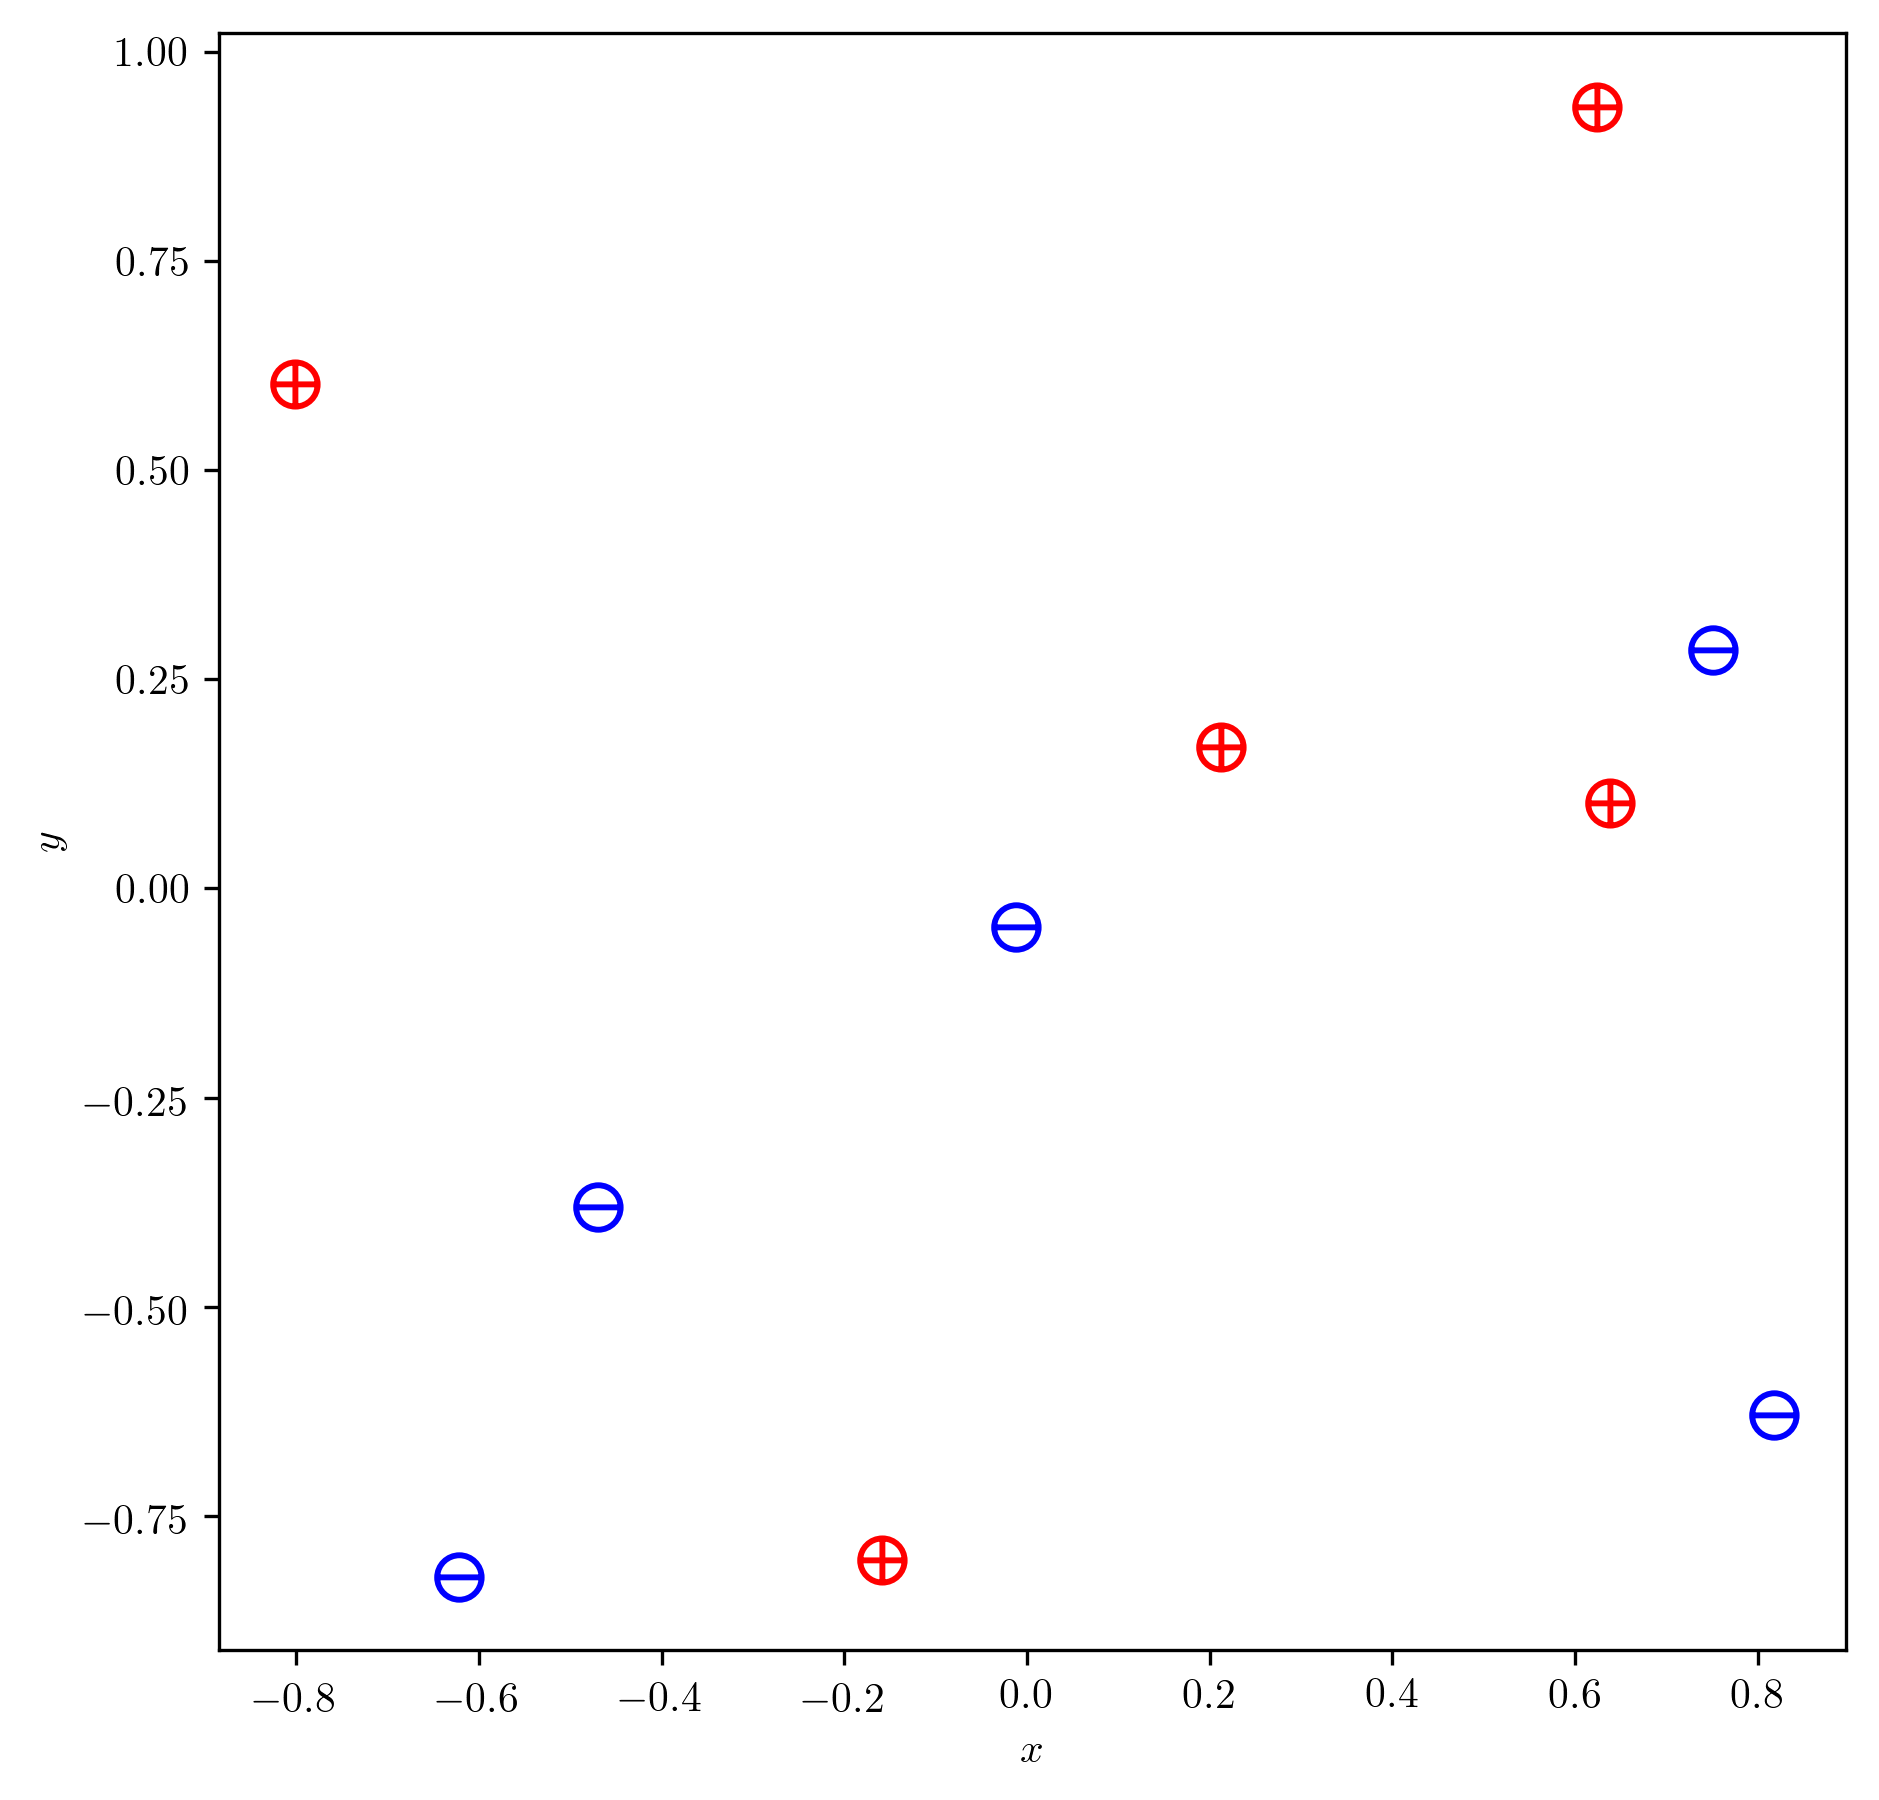
\includegraphics[width=\textwidth]{113.png}
		\caption{}
		\label{fig:plane}
	\end{subfigure}
	\begin{subfigure}[h!]{0.45\textwidth}
		\centering
		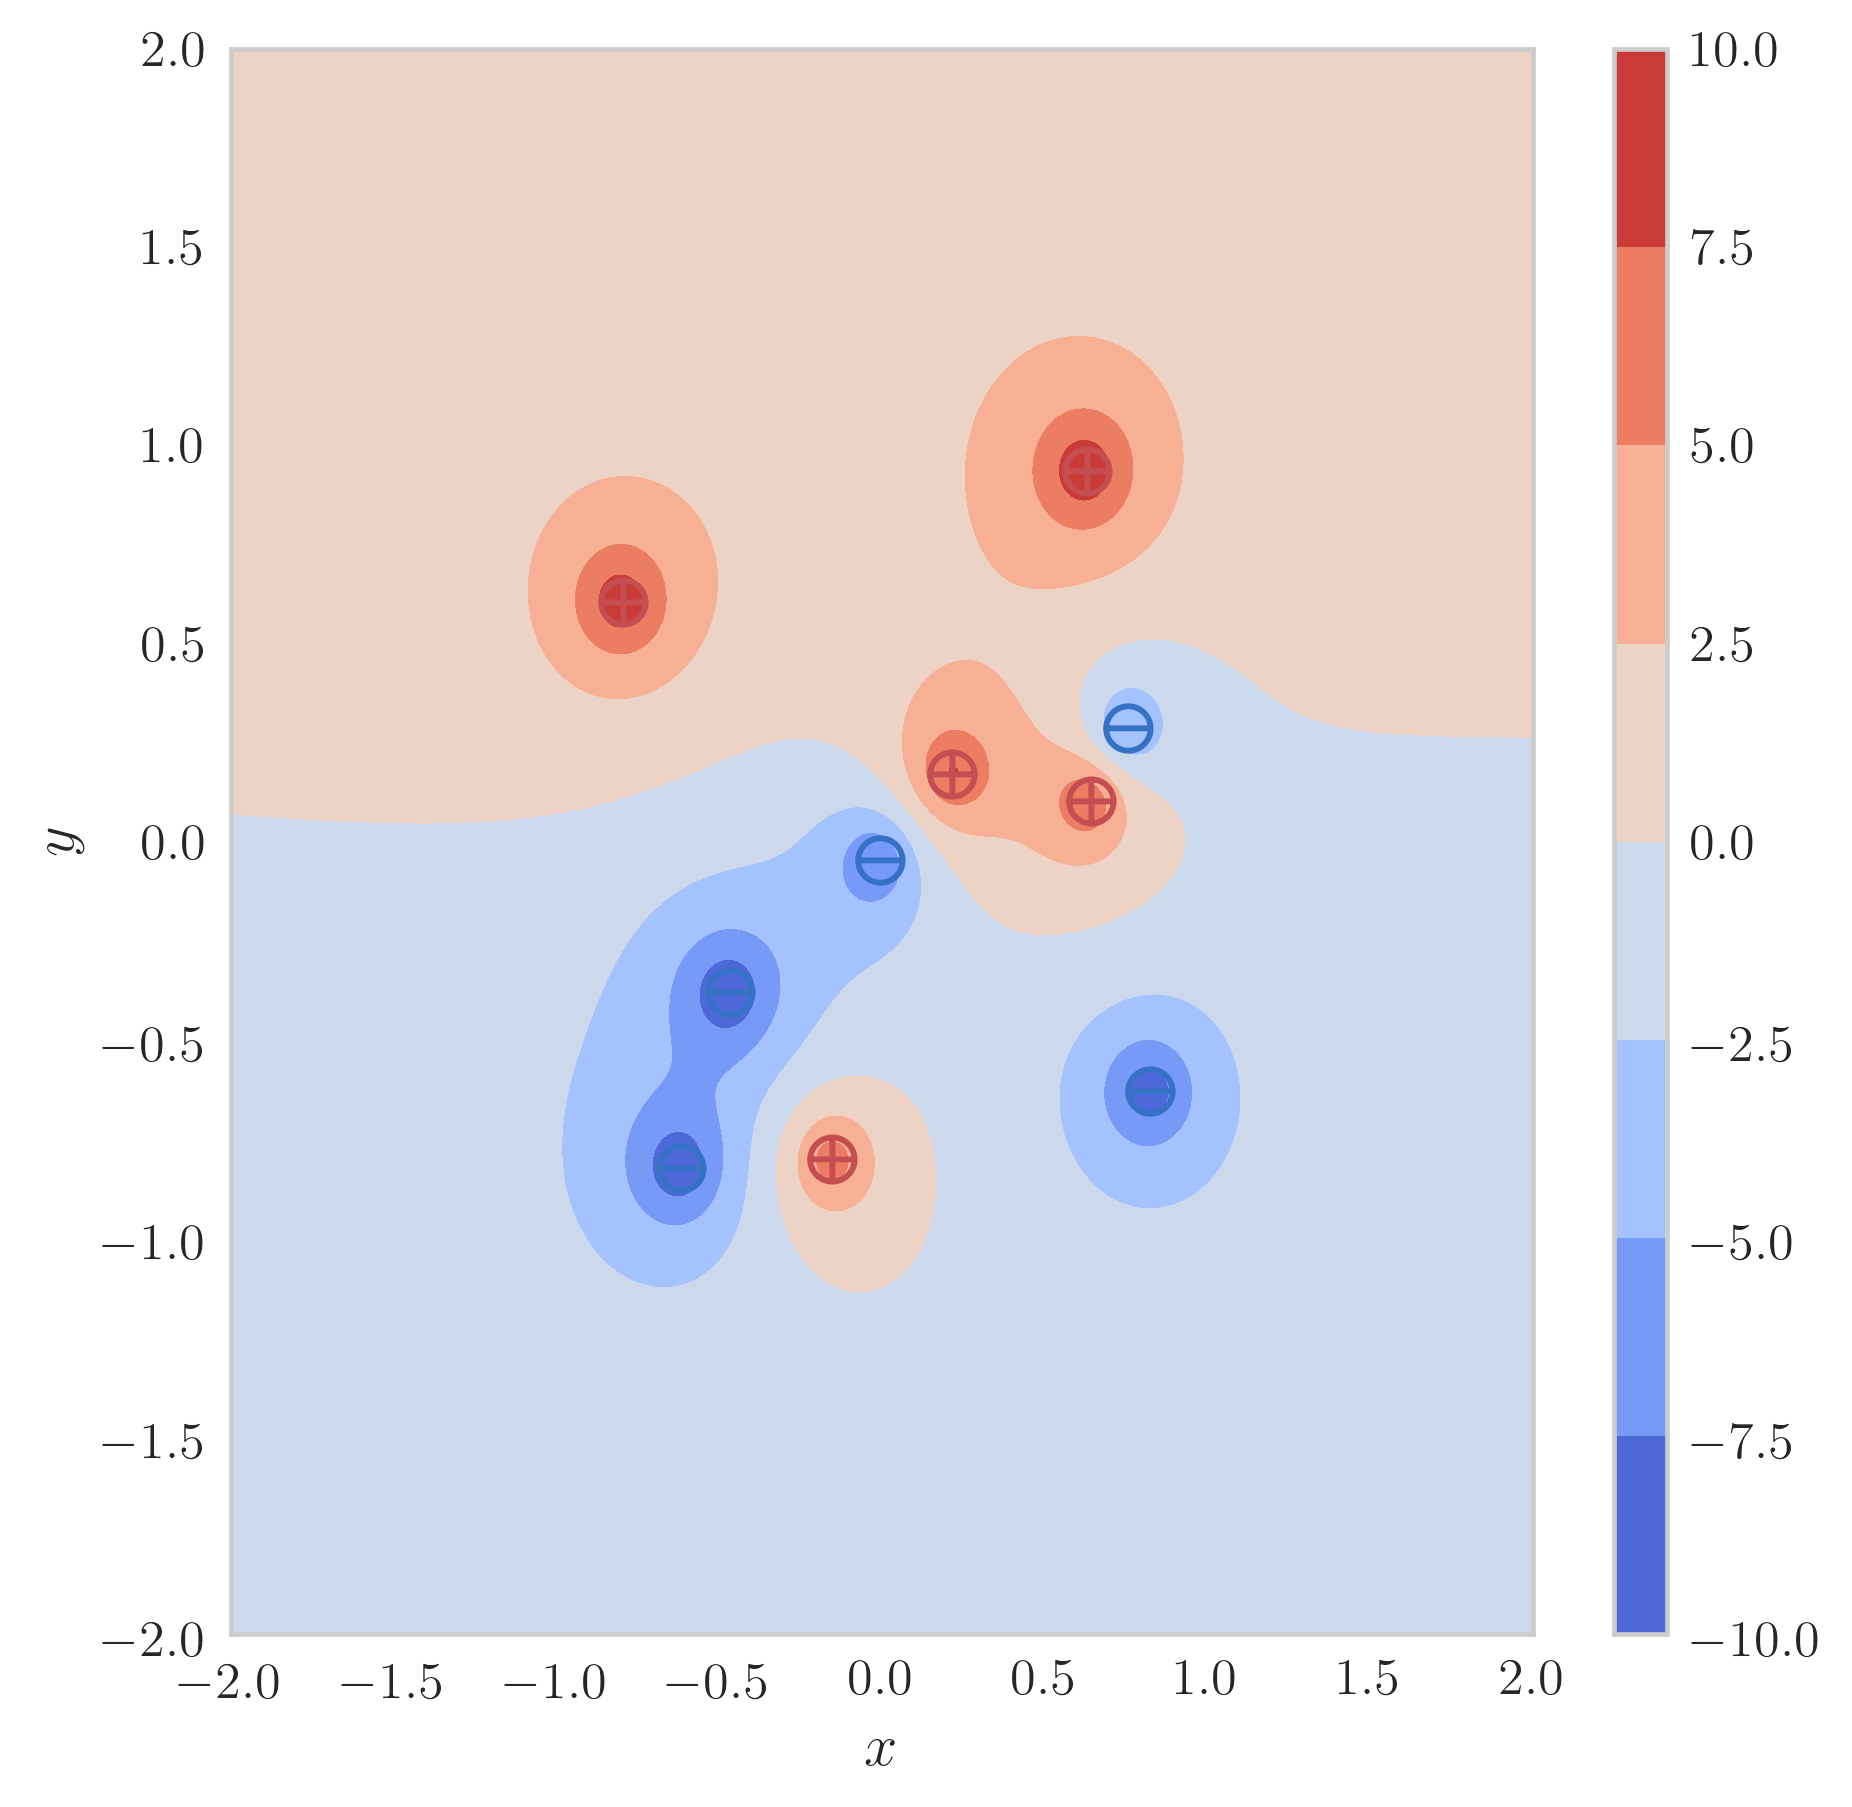
\includegraphics[width=\textwidth]{115.png}
		\caption{}
		\label{fig:contour}
	\end{subfigure}
	\caption{(a) Random distribution of charges on the $x$-$y$ plane. (b) Potential of 10 unit charges on the plane $z=0.1$.}
	\label{fig:projections}
\end{figure}

With the random seed fixed for reproducibility, all the pre-execution code was defined as a \texttt{MultipoleExpansion} class that takes an arbitrary even number $N$ of charges as the sole argument. The behavior of the electrostatic potentials and fields was investigated by generating $N$ unit point charges, scattered within a $2 \times 2$ meter box on the $x$-$y$ plane, centered at the origin. Random numbers were then drawn from a uniform distribution and inserted into the row vectors of an array \texttt{r}. Thus, \texttt{r} is a $3 \times N$ matrix, with the rows representing the position vectors of the charges and all the $z$-components set to zero. From these vectors, the first half were assigned to be the positive charges, while the latter half were assigned as the negative charges.

The electric potential was calculated for a $4 \times 4$ meter box on the $x$-$y$ plane by dividing it into a $500 \times 500$ \texttt{meshgrid} for $x,y \in [-2,2]$, then evaluating the exact $\Phi$ for each point in the meshgrid using \eqref{eq:potential}, and setting units of $4\pi\epsilon_0 = 1$. The potential was then plotted as a contour projection on the $x$-$y$ plane using the \texttt{Axes3D} object \cite{matplotlib}. To quantify the accuracy of the dipole and quadrupole approximations, the potential was also plotted as a function of $y$ using the dipole and quadrupole approximations given by \eqref{eq:multipole}, superimposed with the exact potential given by \eqref{eq:potential}.

Finally, the electric field was numerically evaluated using the central difference algorithm, as defined in \cite{wilmott}\cite{olver}, and was plotted using \texttt{streamplot} \cite{christian}.

\section{Results}
\label{sec:RnD}
\medskip

\begin{figure}[tb]
	\centering
	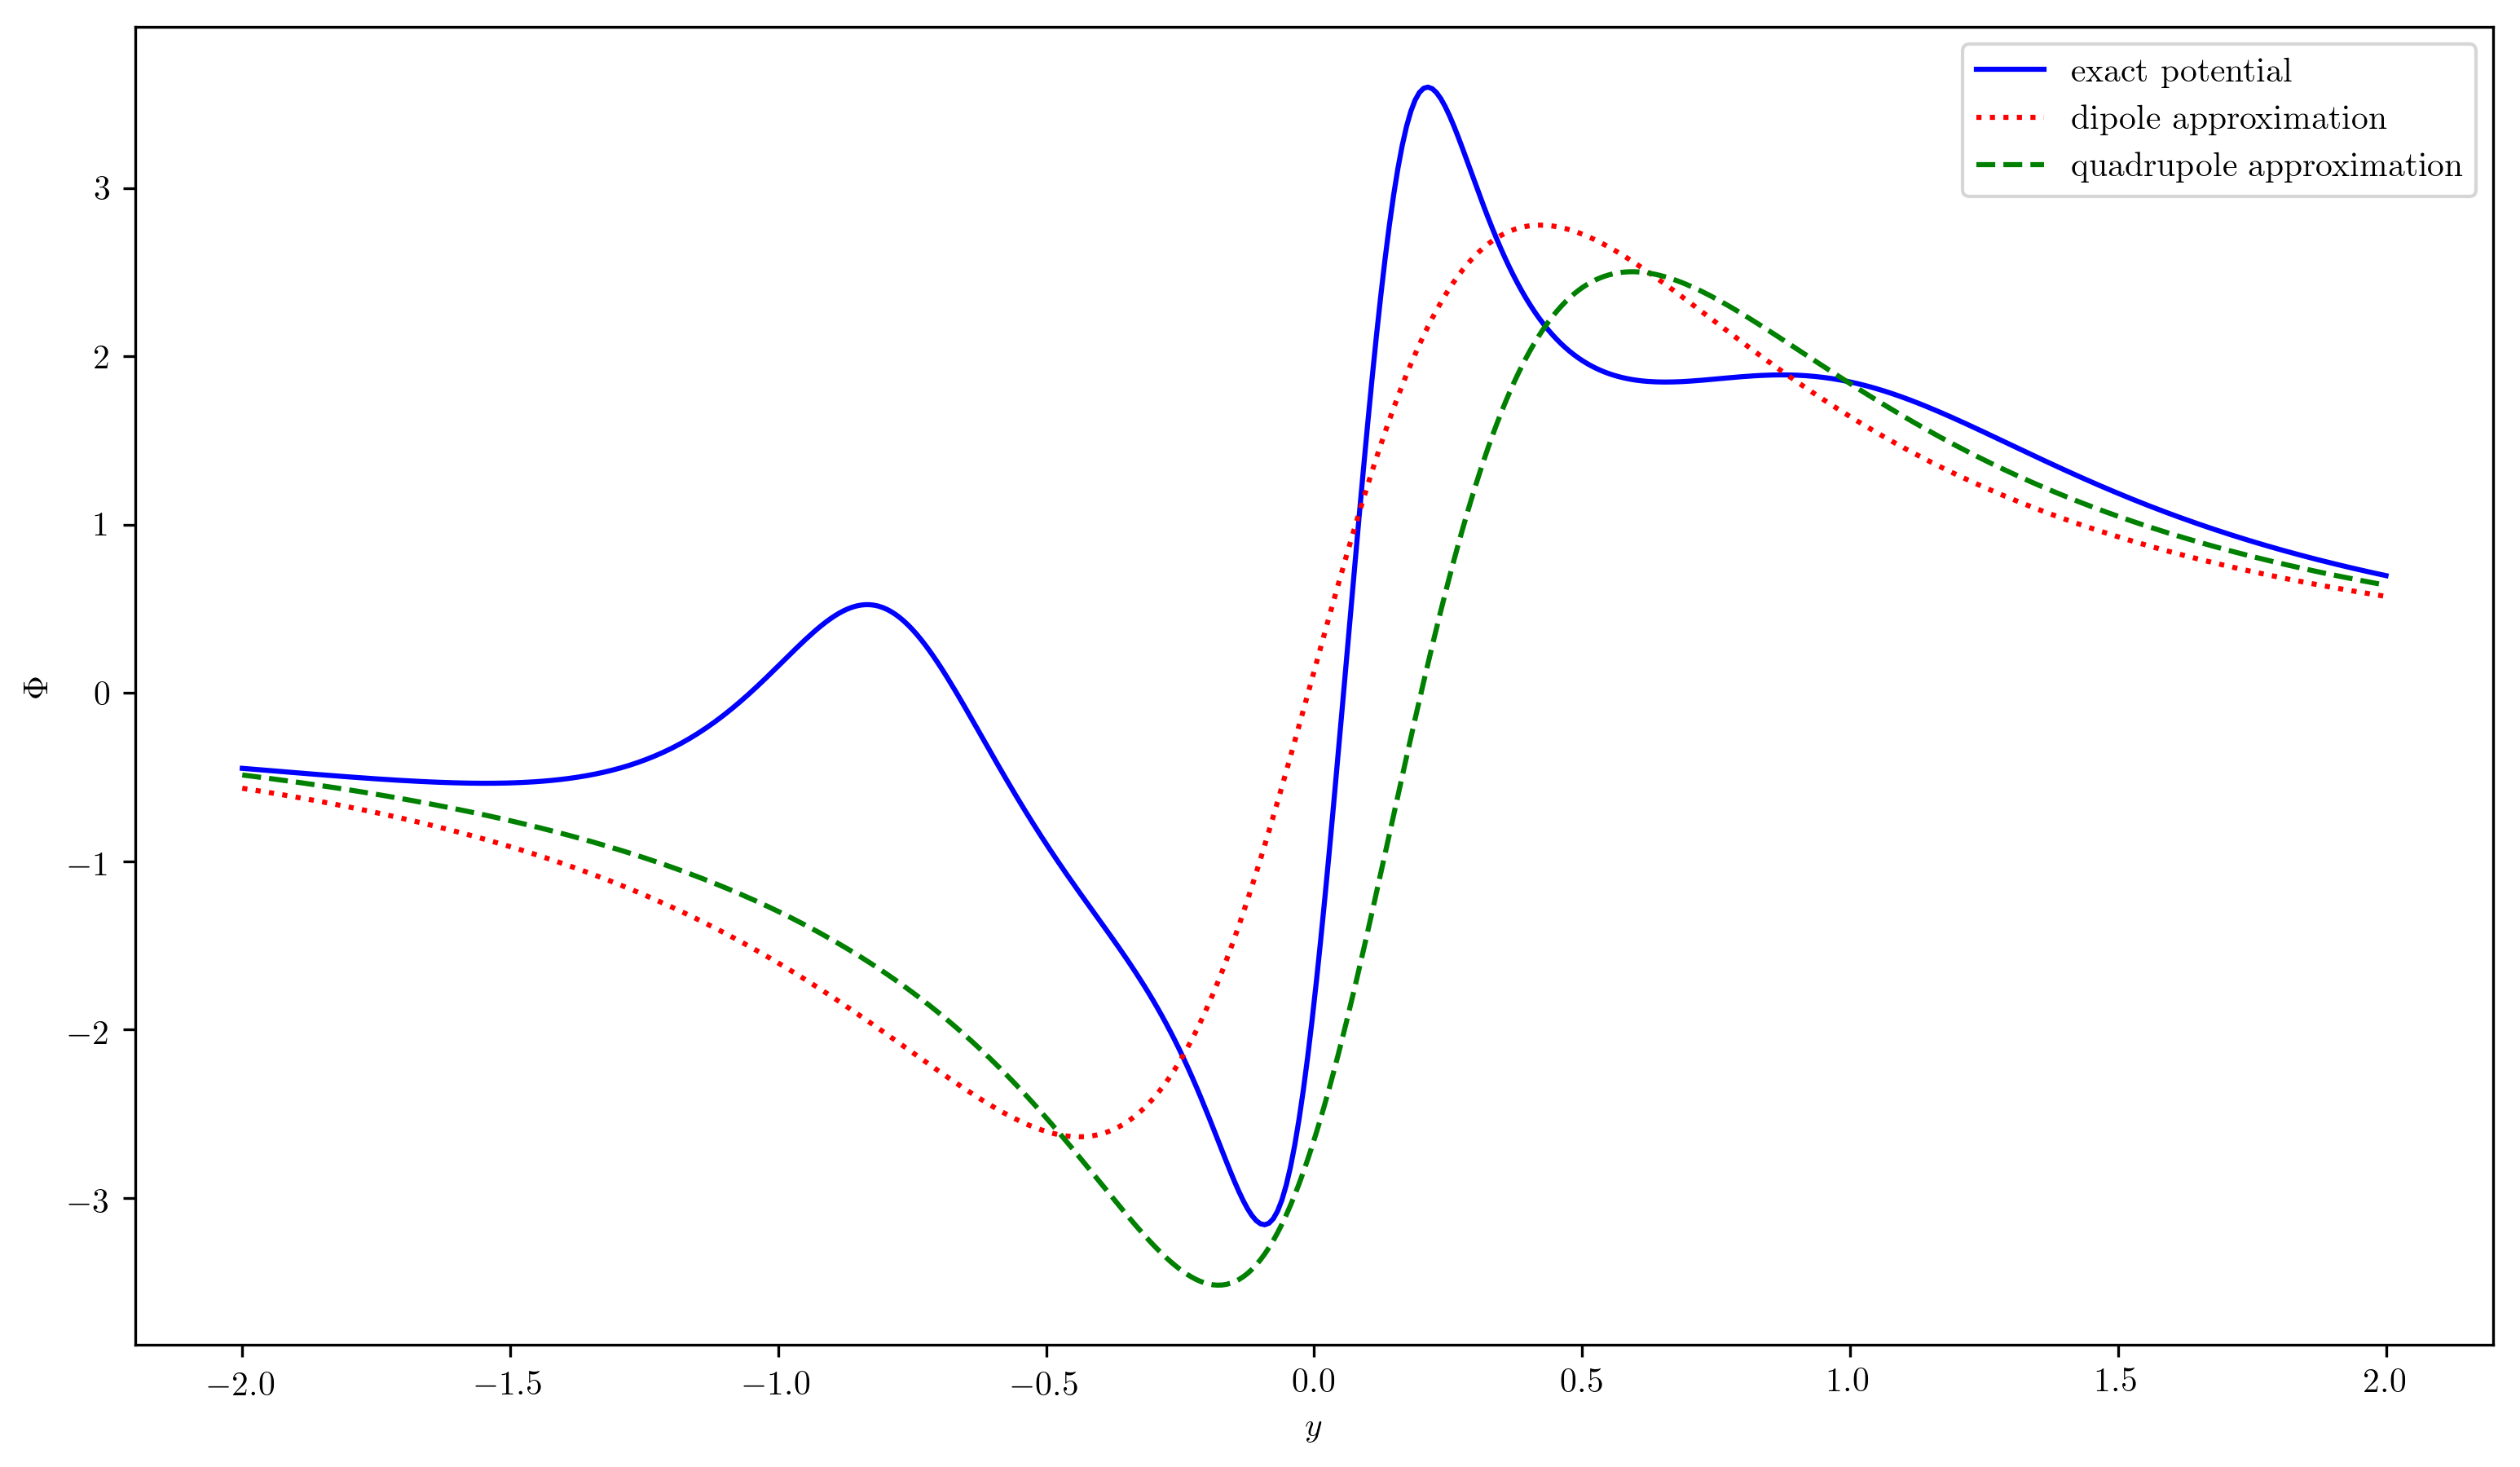
\includegraphics[width=0.74\textwidth]{116.png}
	\caption{Potentials for different approximations at $x = z = 0.1$.}
	\label{fig:approx}
\end{figure}

A total of ten (10) point charges were generated for the purposes of this paper. Their distribution on the $x$-$y$ plane is shown in Figure \ref{fig:plane}. On the plane $z = 0.1$, they generate a potential, which is shown as contours of constant $\Phi$ in Figure \ref{fig:contour}.

To compare the dipole and quadrupole approximations to the exact potential, a plane parallel to the $y$-axis was selected and ``cut'' at the location $x = z = 0.1$. This plane was of particular interest due to the fact that it passes close to two positive charges at $y \approx \pm 1$, and runs right in the middle of a dipole near $y \approx 0$. Figure \ref{fig:approx} shows the result. It can be observed that the dipole approximation cannot account for both of the positive charges on either side of the origin. This is due to the fact that the dipole approximation only allows for two turning points in its curve. Even with the quadrupole correction, the actual potential is emulated only in a very rough manner.

Calculation of the electric field yields the graphs in Figure \ref{fig:field}. Figure \ref{fig:field-2m} shows the complex structure of the electric field for multiple charges, and as one moves away from the charge distribution, the field appears to be that of a dipole, as can be seen in Figure \ref{fig:field-64m}.

\begin{figure}[tb]
    \centering
	\begin{subfigure}[h!]{0.45\textwidth}
		\centering
		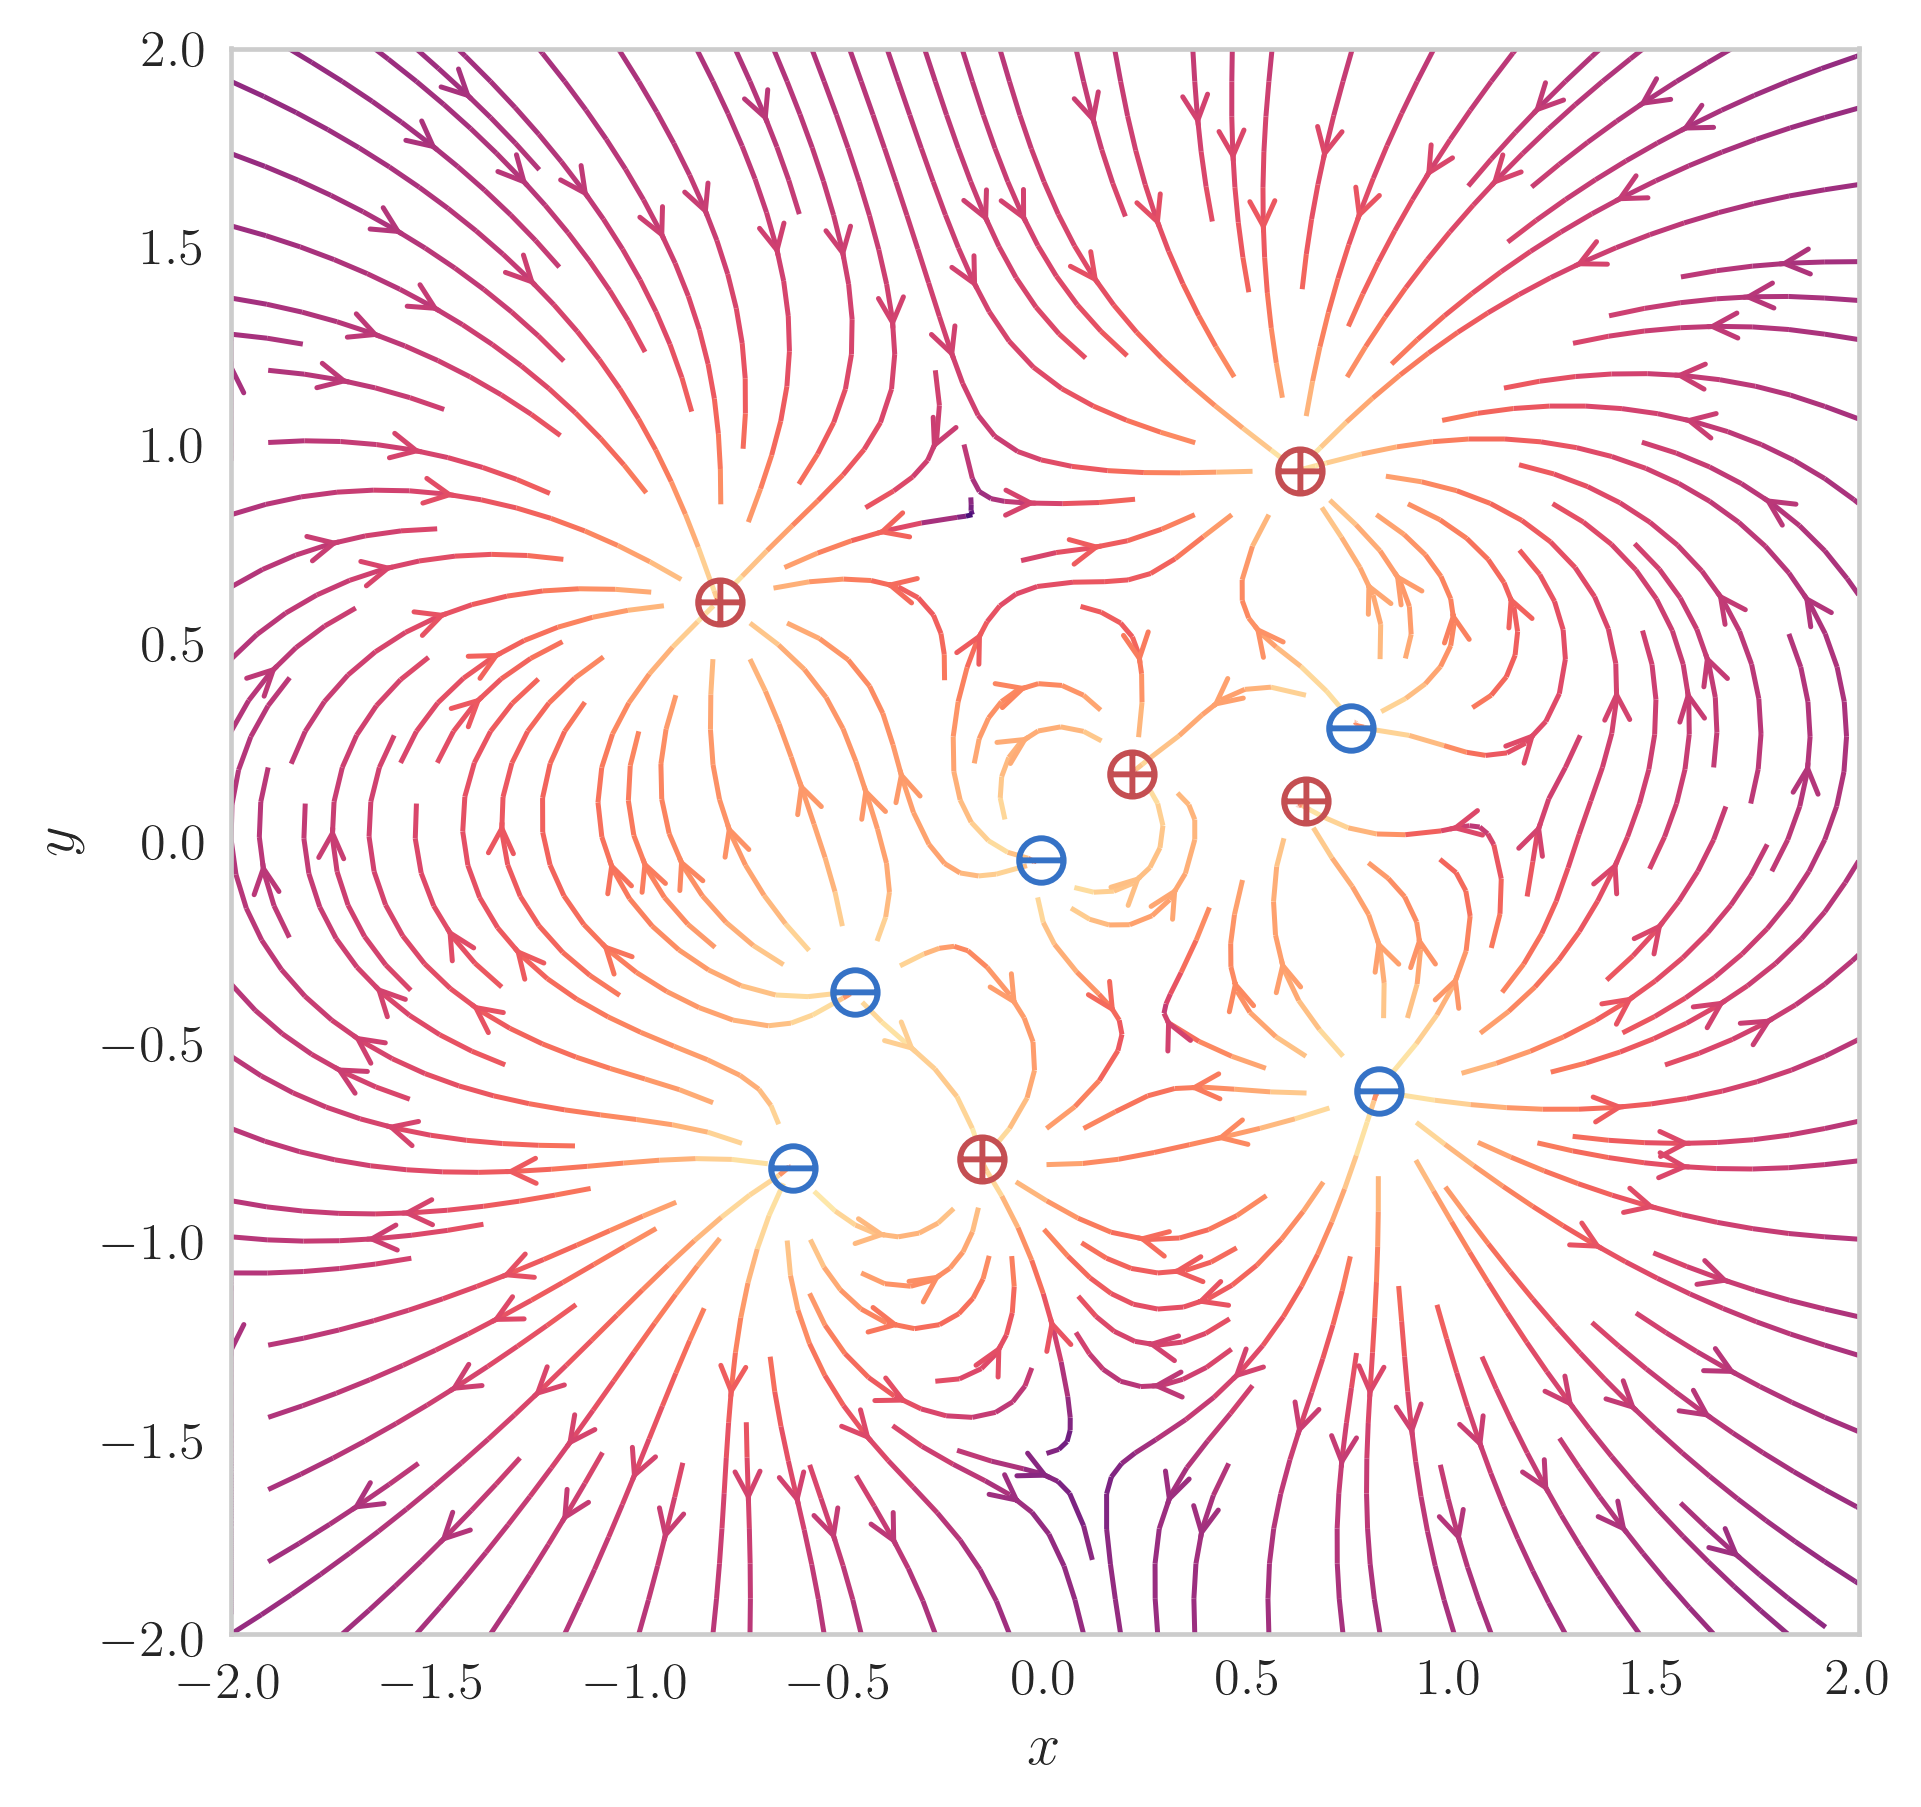
\includegraphics[width=\textwidth]{117-2.png}
		\caption{}
		\label{fig:field-2m}
	\end{subfigure}
	\begin{subfigure}[h!]{0.45\textwidth}
		\centering
		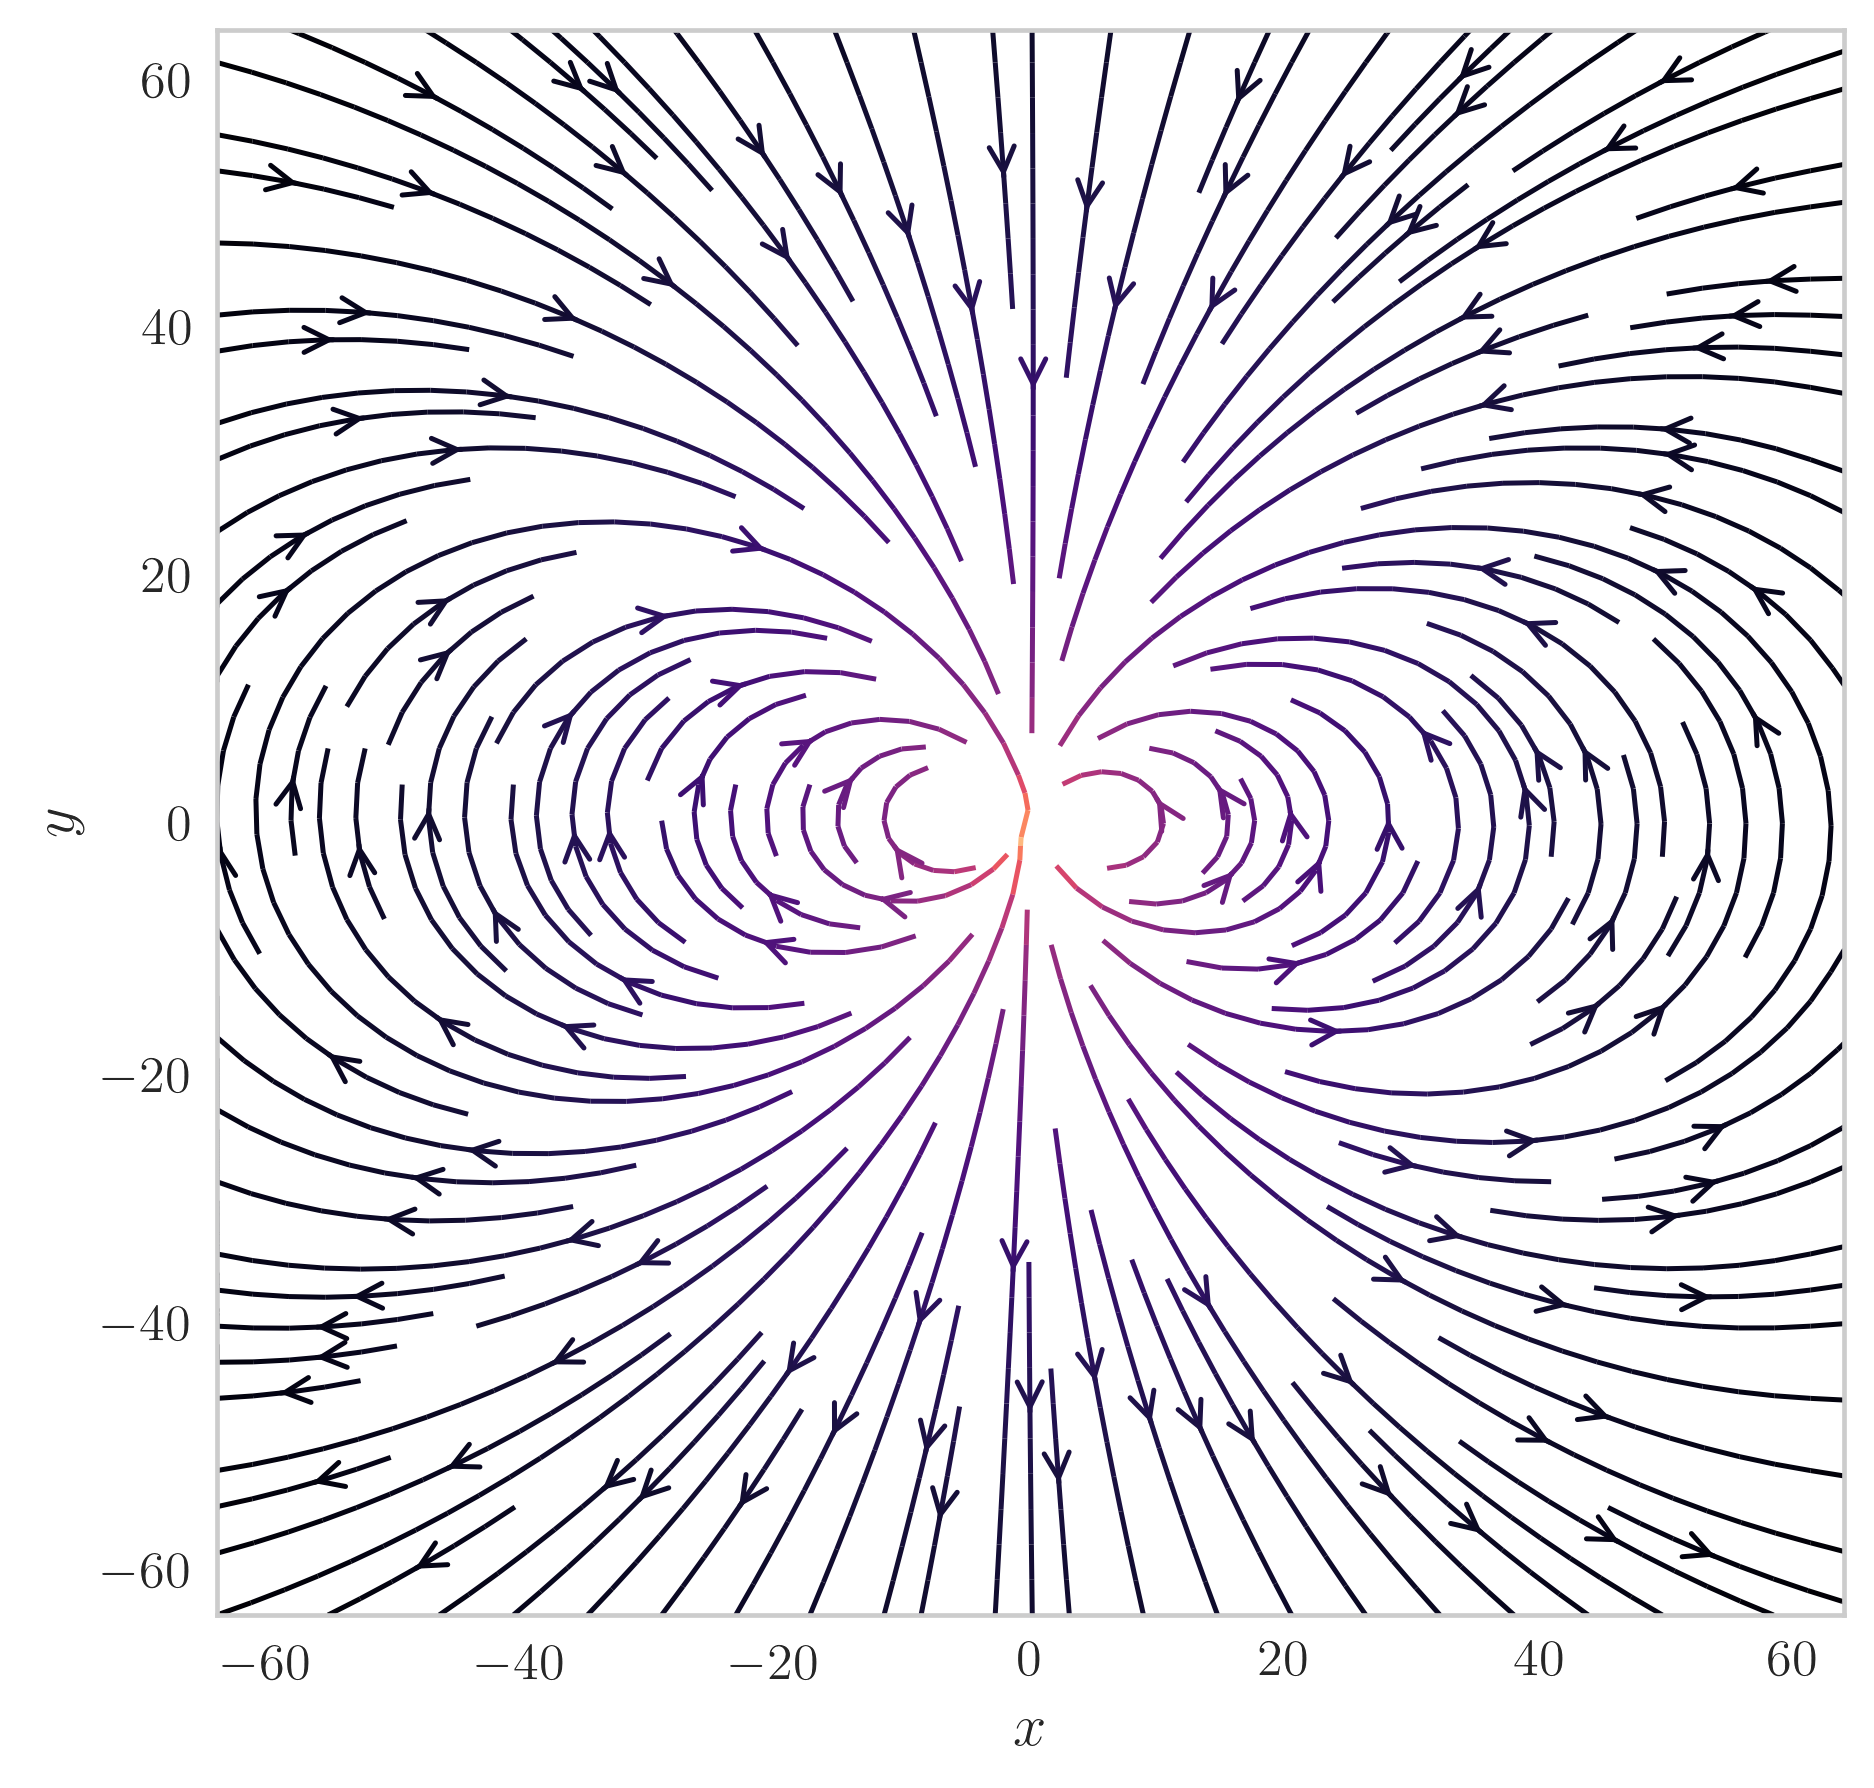
\includegraphics[width=\textwidth]{117-64.png}
		\caption{}
		\label{fig:field-64m}
	\end{subfigure}
	\caption{Electric field of 10 unit charges viewed at (a) 2 m, and (b) 64 m away from the charge distribution.}
	\label{fig:field}
\end{figure}

\bibliographystyle{spp-bst}
\begin{thebibliography}{1}
\label{sec:Ref}

\bibitem[Kinzel(1998)]{kinzel}
Kinzel, W., and G. Reents (1998). Multipole expansion. In M. Clajus, and B. Freeland-Clajus (Trans.), \textit{Physics by computer: programming physical problems using Mathematica and C}, pp. 30-36. New York: Springer (Original work published 1996).

\bibitem[Griffiths(1999)]{griffiths}
Griffiths, D.J. (1999). Multipole expansion. \textit{Introduction to electrodynamics} (3rd ed.), pp. 146-159. New Jersey: Prentice-Hall.

\bibitem[Gradshteyn and Ryzhik(1994)]{gradshteyn}
Gradshteyn, I.S., and I.M. Ryzhik. (1994). \textit{Table of integrals, series, and products}. Boston, MA: Academic Press.

\bibitem[Hunter(2007)]{matplotlib}
Hunter, J.D. (2007). Matplotlib: a 2D graphics environment. \textit{Computing in science and engineering \textbf{9}}(3), 90-95.

\bibitem[Wilmott et. al.(1995)]{wilmott}
Wilmott, P., S. Howison, and J. Dewynne. (1995). \textit{The mathematics of financial derivatives: a student introduction}, p. 137. Cambridge University Press.

\bibitem[Olver(1995)]{olver}
Olver, P. (2013). \textit{Introduction to partial differential equations}, p. 182. Springer Science \& Business Media.

\bibitem[christian(2015)]{christian}
christian. (2015, 10 December). Visualizing a vector field with Matplotlib. Retrieved 12 October 2018, from \textit{Learning scientific programming with Python}: \url{https://scipython.com/blog/visualizing-a-vector-field-with-matplotlib/}.

\end{thebibliography}

\end{document}
